%%% LaTeX Template: Article/Thesis/etc. with colored headings and special fonts
%%%
%%% Source: http://www.howtotex.com/
%%% Feel free to distribute this template, but please keep to referal to http://www.howtotex.com/ here.
%%% February 2011
%%%
%%% Last updated September 2018 by CDM

%%%  Preamble
\documentclass[11pt,letterpaper]{article}
\usepackage[margin=1.0in]{geometry}
\usepackage[T1]{fontenc}
\usepackage[bitstream-charter]{mathdesign}
\usepackage[latin1]{inputenc}					
\usepackage{amsmath}						
\usepackage{xcolor}
\usepackage{cite}
\usepackage{hyphenat}
\usepackage{graphicx}
\usepackage{float}
\usepackage{subfigure}
\usepackage{sectsty}
\usepackage[compact]{titlesec} 
\usepackage[tablegrid]{vhistory}
\allsectionsfont{\color{accentcolor}\scshape\selectfont}

%%% Definitions
\definecolor{accentcolor}{rgb}{0.0,0.0,0.5} 
\newcommand{\teamname}{UTASC}
\newcommand{\productname}{UTA Summer Conferences Manager}
\newcommand{\coursename}{CSE 4316: Senior Design I}
\newcommand{\semester}{Fall 2018}
\newcommand{\docname}{Project Charter}
\newcommand{\department}{Department of Computer Science \& Engineering}
\newcommand{\university}{The University of Texas at Arlington}
\newcommand{\authors}{Pavanaj Biyani \\ Robert Brady \\ Brandon Chase \\ Kartik Gupta \\ Nicholas Reimherr}

%%% Headers and footers
\usepackage{fancyhdr}
	\pagestyle{fancy}						% Enabling the custom headers/footers
\usepackage{lastpage}	
	% Header (empty)
	\lhead{}
	\chead{}
	\rhead{}
	% Footer
	\lfoot{\footnotesize \teamname \ - \semester}
	\cfoot{}
	\rfoot{\footnotesize page \thepage\ of \pageref{LastPage}}	% "Page 1 of 2"
	\renewcommand{\headrulewidth}{0.0pt}
	\renewcommand{\footrulewidth}{0.4pt}

%%% Change the abstract environment
\usepackage[runin]{abstract}			% runin option for a run-in title
%\setlength\absleftindent{30pt}			% left margin
%\setlength\absrightindent{30pt}		% right margin
\abslabeldelim{\quad}	
\setlength{\abstitleskip}{-10pt}
\renewcommand{\abstractname}{}
\renewcommand{\abstracttextfont}{\color{accentcolor} \small \slshape}	% slanted text

%%% Start of the document
\begin{document}

%%% Cover sheet
{\centering \huge \color{accentcolor} \sc \textbf{\department \\ \university} \par}
\vspace{1 in}
{\centering \huge \color{accentcolor} \sc \textbf{\docname \\ \coursename \\ \semester} \par}
\vspace{0.5 in}
\begin{figure}[h!]
	\centering
   	
\includegraphics[width=0.60\textwidth]{images/SummerConferences}
\end{figure}
\vspace{0.5 in}
{\centering \huge \color{accentcolor} \sc \textbf{\teamname \\ \productname} \par}
\vspace{0.5 in}
{\centering \large \sc \textbf{\authors} \par}
\newpage


%\vspace{1 in}
%\centerline{October 1st, 2018}
%\newpage

%%% Revision History
\begin{versionhistory}
  	\vhEntry{0.1}{10.01.2018}{GH}{document creation}
  	\vhEntry{0.2}{10.05.2018}{AT|GH}{complete draft}
  	\vhEntry{0.3}{10.12.2018}{AT|GH}{release candidate 1}
  	\vhEntry{1.0}{10.20.2018}{AT|GH|CB}{official release}
  	\vhEntry{1.1}{10.31.2018}{AL}{added customer change requests}
\end{versionhistory}
\newpage

%%% Table of contents
\tableofcontents
\newpage

%%% List of figures and tables (optional)
\listoffigures
%\listoftables
\newpage
\setcounter{table}{0}

%%% Agile project charter sections
\section{Vision}
UTA Summer Conferences hosts close to 100 camps over the summer. They have a revenue loss of approximately $50,000 every summer because of the current system of loosely tied applications and human error in using those applications. By providing a streamlined one-stop solution for them to manage all the tasks, from requesting to host a camp to billing, we would save a lot of time and money of the department.
\section{Mission}
Our mission is to replace the old system followed by UTA Summer Conferences with a full stack web application which they can access from any machine on UTA Campus. Our goal is to build an application that manages all aspects of summer camps and conferences, viz. booking requests, billing, equipment, check-in & check-out, parking, linens, room reservations, etc. We will provide an easy to use UI which communicates with the backend database via API requests.
\section{Success Criteria}
The success criteria are enumerated effects outside of the development of the solution (i.e., NOT specific project requirements) that can be observed and measured to quantify "what success looks like". The key is to focus on specific expected benefits beginning immediately after the project is delivered and projecting forward into the future. Bullet lists should be used to itemize each success criterion, and each item should have a time frame and some sort of quantifiable measurement.

One way to list the success criteria is to use lists for different time frames. Here is a short example:
\\
\\
Upon completion of the prototype system, we expect the following success indicators to be observed on kiosk stations implementing the new GUI software:
\begin{itemize}
  \item A 10\% reduction in operating costs
  \item 30\% reduction in average transaction time
  \item 20\% increase in mean time to failure (MTTF)
\end{itemize}

Within 6 months after the prototype delivery date, we expect the following success indicators to be observed:
\begin{itemize}
  \item An additional 10\% reduction in operating costs
  \item An additional 10\% reduction in average transaction time
  \item An additional 5\% increase in mean time to failure (MTTF)
\end{itemize}

Within 12 months after the prototype delivery date, we expect the following success indicators to be observed:
\begin{itemize}
  \item Expansion of the system to 3 additional deployment sites
  \item Porting of the system to additional hardware platforms, such as Super Kiosk and Alpha Pay
  \item An additional 15\% reduction in operating costs
\end{itemize}
\\
\\
NOTE: The vision, mission, and success criteria, when combined, should occupy \underline{EXACTLY ONE FULL PAGE}. This can be individually distributed as an agile project charter or executive summary when necessary. 
\\
NOTE: Throughout the document, remove and replace all instruction text with your own material. 

\newpage

%%% Remaining project charter sections
\section{Background}
The University of Texas at Arlington hosts summer camps during the summer months of May, June, July, and August ranging from organizational to religious camps. To register, accommodate their stay, and bill these camps, all their data is stored on Google Sheets in a variety of tabs. This include contract information, rosters, checked out equipment, stay durations, parking, work orders, and billing. By manipulating permissions to establish a five-tier hierarchy, that of administrators, professional staff, residence directors, resident assistants, and camp coordinators, where each group will have different permissions within the set of sheets. Since the data stored in Google Sheets is not covered under FERPA, it can be legally stored in this public manner but is encountering several issues. First, there can be upwards to thirty employees, masked behind their respective titles, touching the Google Sheet without individually identifying themselves. Therefore, data can be edited and deleted at whim without knowing who was responsible for it. Second, human error has led to an estimated loss of 50,000 over the past three months. This includes incorrect check-in/check-out dates for campers, forgetfulness in duplicate manual entries, and an inability to utilize all open residence hall rooms. Third, staff members are triple checking both the inputted data in Google Sheets and their hall cards, keys, and temporary cards to ensure that they are in order whereas most of these processes can be automated. Lastly, the administration spends several hours a week managing permissions for each sheet (it is not unusual to have up to 15 sheets per camp), ensuring that the five-tier hierarchy remains in place for each camp.
The business case for this system will begin when a camp requests to stay at UTA. The gathering of basic information, such as the number of bed spaces, duration, extra meeting spaces, dining, linens, etc., will be collected. Upon preliminary approval, legal paperwork will need to be filled out that outlines a contract between the camp director and UTA. Just prior to the camp arriving, the roster including all names of the campers will need to be uploaded. On check-in, campers, camp counselors, and camp coordinators will need to be assigned to a specific bed space, given a respective magnetic strip card and hard key for their room and accommodate parking. It is possible that during a stay, a maintenance emergency happens such that multiple campers may need to move rooms and a work order needs to be submitted. Additionally, campers may want to check out recreational equipment for billiards, table tennis, or video game consoles. If any of these items are damaged or lost, these details should be noted. Upon check-out, all magnetic cards, hard keys, and card holders need to be returned and assessed for damages. Any keys lost or damaged should be noted for billing purposes. After a camp has completed their stay, the used rooms need to be checked for any damages, cleaned, and finally set back up for the following camp. Any damages found inside the rooms will need to be noted for billing purposes. Finally, once it is time to bill a camp, a grand total will be calculated from the number of used bed spaces, their duration, parking, damaged equipment, damaged cards, extraneous meeting spaces, dining, linens, etc. If desirable, a payment confirmation can be uploaded for filing purposes.
This project will add tremendous value to UTA Summer Conferences, allowing for less human error, increased efficiency, eliminating several manual processes, and increasing UTA’s professional public appearance. As this project will come at no charge to their organization, Summer Conferences is excited to have a custom system that will accommodate all of their needs.

\section{Related Work}
In general, most off-the-shelf solutions are not sufficient since they are not tailored to the process that is used to manage the UTA Summer Conferences. For example, UTASC will handle the systems behind scheduling a camp, using key cards to check in and out of rooms as well as check in and out equipment, handle parking and directly communicate with the UTA parking system, integrating directly into the specific floor plans of the dorm halls at UTA, and managing the various levels of permissions. 
In addition, there are various other specific things that our customer needs UTASC to do that either aren't done in other solutions, don't integrate well with the other systems in UTASC, or are too expensive. In short, our project has merit because we can cheaply provide a very tailored-fit, tightly integrated software solution that covers all our customer's needs, which can't be met with other related works.
The first related work is the Abacre Hotel Management System. It is "a complete hotel management system that begins with taking the guest reservations and check in / check out and ends with billing and tax reports" \cite{website:abacre}. This would only useful for the room check in / check out system. 
The next related work is KWHotel. It is a "hotel management software designed for small and medium accommodation facilities" cite{website:kwhotel}. Again, its functionality is quite limited compared to what we will need to implement for our customer.
Another related work is EZ Rent Out. It is used for renting out equipment, but it has many more features than is needed for our use case. It is also very expensive at \$ 50 per month for the cheapest option and \$ 20 more per additional user cite{website:ezrentout}.
For parking, an existing commercial solution is BOSSCARS. "Tailored to meet the unique needs of colleges and universities, BOSSCARS parking permit software was specifically designed to manage all aspects of parking operations, promote better customer service, and increase revenues" cite{website:bosscars}. This would act as a standalone system, kind of like to replacing UTA's existing system. We just need something that is able to hook into UTA existing parking system and send requests for temporary permits.
Lastly, there is Guest Tracker for room key card management software. "Information including room number, length of stay, and checkout date and time is automatically transferred" to the front desk station cite{website:guesttracker}. This isn't viable since it requires the user to install their custom door handles and use their custom keys while we require a solution that already integrates with their current keycard system. Also, it is very expensive at about \$ 10,000 for enough licenses for the various rooms we are handling.

\section{System Overview}
This section should reintroduce the full data flow diagram from the architectural specification, and discuss at a high level the purpose of each layer. You do not need to include a subsection for each layer, a 1 - 2 paragraph recap is sufficient.

\begin{figure}[h!]
	\centering
 	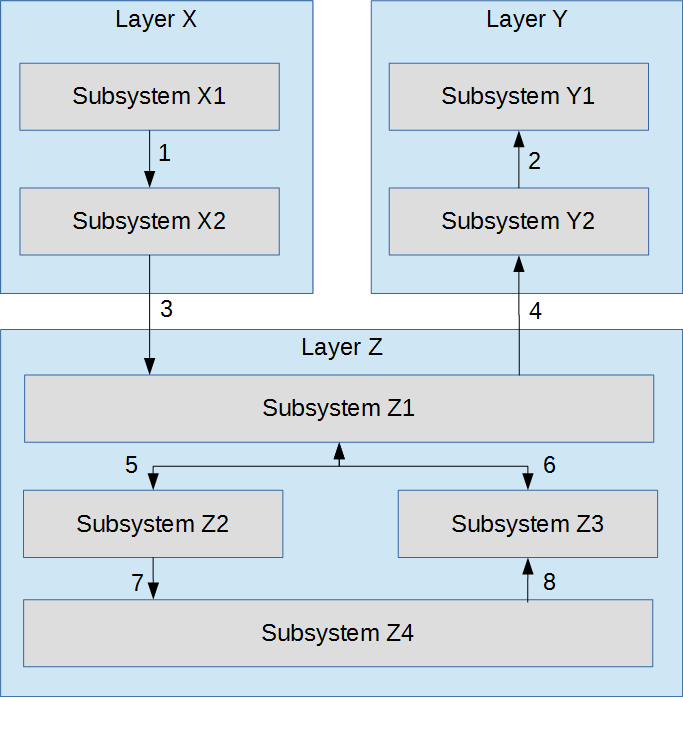
\includegraphics[width=0.90\textwidth]{images/data_flow}
 \caption{System architecture}
\end{figure}

\section{Roles \& Responsibilities}
Who are the stakeholders of the project? Who will be the point of contact from the sponsor or customer side? Who are the team members, and what will be their areas of responsibility? Will your team maintain the product owner and scrum master for the whole project, or will that role change periodically? This section should occupy 1/2 - 1 full page.
\section{Cost Proposal}
This section contains the approximate budget for the project, where that money will come from, and any other support. This text should be replaced with a discussion and justification of major expenses, but not the actual monetary amounts (that will go in the preliminary budget section below). 

\subsection{Preliminary Budget}
Include a high level budget table for components, fabrication, software licensees, development hardware, etc. 

\subsection{Current \& Pending Support}
What are all of the funding sources for the project, and are there any potential funding sources that haven't been secured yet? List all funding sources (including the default funding amount provided by the CSE department) and their dollar amounts.
\section{Facilities \& Equipment}
What lab space, testing grounds, makerspaces, etc. will you need to complete the project? Will you require any specific equipment, and if so, where will you get it (borrow, lease, purchase, outsource, already present in the lab, etc.). This section should occupy 1/2 page.
\section{Assumptions}
\begin{itemize}
  \item The UTA Summer Conferences Director, Kirstin Coffman, is assumed to be available to meet with at least once per sprint. It is critical that Kirstin be able to prioritize the features that are most crucial to the system in the event that there is not enough time to finish the project. This assumption includes an average response rate to email to set up meetings.
  
  \item The second assumption is that during our data gathering phase we will have access to the physical camper cards and hard keys to retrieve their PIK numbers and key numbers. We are also assuming that we will have access to the floor plans to model the building digitally. Lastly, we expect to be provided with the card readers that are already programmed to accept the magnetic cards.
  
  \item For authentication into the system, we are assuming that we will either be expected to use UTA’s netID and password or integrate with ‘Sign in with Google’ or ‘Sign in with Microsoft’ so that the software will not have to manage both users, their passwords, and security.
  
  \item One of our major assumptions is that the system will be able to talk with other services on campus through APIs that are crucial to the summer conferences operations. These services include work orders managed by UTA Maintenance, EMS which is scheduling software to book campus meeting rooms and residence hall rooms, and UTA Parking to add guest license plates to UTA's systems so that they do not get charged.
  
  \item Lastly, an assumption is that UTA will allow Summer Conferences to use the software even if it is not residing on UTA servers. As this system will be hosted on a cloud platform managed by large corporations, it will not be managed by UTA.
  \end{itemize}
  
\section{Constraints}
The following list contains key constraints related to the implementation and testing of the project.

\begin{itemize}
  \item The project must be finished by the end of the 2019 Spring semester
  \item The total development costs must not exceed \$800 for the project unless we find a sponsor. This will likely be used to pay for hosting the web server and any possible software developer licenses
  \item There is a limited amount of time that we can dedicate to the project per week since we have also have to perform work for other classes
  \item Once we graduate we will no longer be able to provide customer support and ongoing maintenance
  \item Our system must integrate with existing UTA systems such as its parking system and its key card system for opening rooms and checking out equipment
\end{itemize}

\section{Risks}
The following high-level risk have been identified in the project, they are ranked in descending order with the highest exposure. Mitigation strategies will be discussed in future planning sessions. We have identified some scheduling risks, some technical & functional risks and some operational and procedural risks.

\begin{table}[h]
\resizebox{\textwidth}{!}{
\begin{tabular}{|l|l|l|l|}
\hline
 \textbf{Risk description} & \textbf{Probability} & \textbf{Loss (days)} & \textbf{Exposure (days)} \\ \hline
Inexperience with implementation tools (Node.js, React) & 0.80 & 20 & 16 \\ \hline
Volatile User Requirements and Specification & 0.50 & 20 & 10 \\ \hline
Inability to capture the scope and domain of the problem & 0.30 & 15 & 5 \\ \hline
Additional documentation required for non-technical users & 0.20 & 20 & 4 \\ \hline
Security Risks when dealing with legal contracts & 0.25 & 10 & 2.5 \\ \hline
\end{tabular}}
\caption{Overview of highest exposure project risks} 
\end{table}

\section{Documentation \& Reporting}
%%% In this section, you will describe all of the various artifacts that you will generate and maintain during the project life cycle. Describe the purpose of each item below, how the content will be generated, where it will be stored, how often it will be updated, etc. Replace the default text for each section with your own description. Reword this paragraph as appropriate.

\subsection{Major Documentation Deliverables}
These deliverables are major grade components of the course. Completing these documents should generally be the sprint goal during the applicable sprint period. Remove this paragraph from your draft, but leave the heading.

\subsubsection{Project Charter}
Describe how this document will be maintained and updated (how often, under what circumstances, etc.). When will the initial version be delivered? When will the final version be delivered?

\subsubsection{System Requirements Specification}
Describe how this document will be maintained and updated (how often, under what circumstances, etc.). When will the initial version be delivered? When will the final version be delivered?

\subsubsection{Architectural Design Specification}
Describe how this document will be maintained and updated (how often, under what circumstances, etc.). When will the initial version be delivered? When will the final version be delivered?

\subsubsection{Detailed Design Specification}
Describe how this document will be maintained and updated (how often, under what circumstances, etc.). When will the initial version be delivered? When will the final version be delivered?

\subsection{Recurring Sprint Items}
The following items will be documented and maintained during each individual sprint. Remove this paragraph from your draft, but leave the heading.

\subsubsection{Product Backlog}
How will items be added to the product backlog from the SRS? How will these items be prioritized? Who makes the decision (product owner, group vote, etc.)? What software will be used to maintain and share the product backlog with team members and stakeholders?

\subsubsection{Sprint Planning}
How will each sprint plan be planned? How many sprints will there be (you need to look at the schedules for this course and previous Senior Design II courses during the appropriate semesters to figure this out).

\subsubsection{Sprint Goal}
Who decides the sprint goal? How will you involve your customer in this process?

\subsubsection{Sprint Backlog}
Who decides which product backlog items make their way into the sprint backlog? How will the backlog be maintained (collaboration software, a "scrum board", etc.)?

\subsubsection{Task Breakdown}
How will individual tasks be assigned from the sprint backlog? Will it be up to each team member to voluntarily claim a task, or will it come from the product owner? How will time spent on tasks be documented?

\subsubsection{Sprint Burn Down Charts}
Who will be responsible for generating the burn down charts for each sprint? How will they be able to access the total amount of effort expended by each individual team member? What format will the burn down chart use (include an example burn down chart below).

\begin{figure}[h!]
    \centering
    
\includegraphics[width=0.5\textwidth]{images/test_image}
    \caption{Example sprint burn down chart}
\end{figure}

\subsubsection{Sprint Retrospective}
How will the sprint retrospective be handled as a team? When will this discussion happen after each sprint? What will be documented as a group and as individuals, and when will it be due?

\subsubsection{Individual Status Reports}
What sort of status will be reported by each individual member, and how often will it be reported? What key items will be contained in the report?

\subsubsection{Engineering Notebooks}
How often will the engineering notebook be updated, at a minimum, by each team member? What is the minimum amount of pages that will be completed for each interval, and how long will that interval be? How will the team keep each member accountable? Who will sign of as a "witness" for each ENB page?

\subsection{Closeout Materials}
The following materials, in addition to major documentation deliverables, will be provided to the customer upon project closeout. Remove this paragraph from your draft, but leave the heading.

\subsubsection{System Prototype}
What will be included in the final system prototype? How and when will this be demonstrated? Will there be a Prototype Acceptance Test (PAT) with your customer? Will anything be demonstrated off-site? If so, will there be a Field Acceptance Test (FAT)?

\subsubsection{Project Poster}
What will be included on the poster, what will be the final dimensions, and when will it be delivered?

\subsubsection{Web Page}
What will be included on the project web page? Will it be accessible to the public? When will this be delivered? Will it be updated throughout the project, or just provided at closeout (at a minimum, you need to provide a simple web page at the end).

\subsubsection{Demo Video}
What will be shown in the demo video(s)? Will you include a B-reel footage for future video cuts? Approximately how long will the video(s) be, and what topics will be covered?

\subsubsection{Source Code}
How will your source code be maintained? What version control system will you adopt? Will source code be provided to the customer, or binaries only? If source code is provided, how will it be turned over to the customer? Will the project be open sourced to the general public? If so, what are the license terms (GNU, GPL, MIT, etc.). Where will the license terms be listed (in each source file, in a single readme file, etc.).

\subsubsection{Source Code Documentation}
What documentation standards will be employed? Will you use tools to generate the documentation (Doxygen, Javadocs, etc.). In what format will the final documentation be provided (PDF, browsable HTML, etc.)?

\subsubsection{Hardware Schematics}
Will you be creating printed circuit boards (PCBs) or wiring components together? If so, list each applicable schematic and what sort of data it will contain (PCB layout, wiring diagram, etc.). If your project is purely software, omit this section.

\subsubsection{CAD files}
Will the project involve any mechanical design, such as 3D printed or laser-cut parts? If so, what software will you use to generate the files and what file formats will you provide in your closeout materials (STL, STEP, OBJ, etc.). If your project is purely software, omit this section.

\subsubsection{Installation Scripts}
How will the customer deploy software to new installations? Will you provide installation scripts, install programs, or any other tools to improve the process? Will there be multiple scripts provided (perhaps separate scripts for the graphical front end and back end server software)? 

\subsubsection{User Manual}
Will you customer need a printed or digital user manual? Will they need a setup video? Decide now what will be provided and discuss.

\newpage

%%% References
\bibliographystyle{plain}
\bibliographystyle{reference/IEEEtran_custom}
\bibliography{reference/refs}{}

\end{document}